% Fig. 4.4 / CH4_FIGURE_SPECS.md line 3418 -- the normal density with the
%   seven boundaries of the empirical rule, mu and mu +- 1, 2, 3 sigma.
% Source: mathstatch4.tex lines 3418-3463.
%
% The manuscript draws 3.069 e^{-(x-4)^2/3} over 0 <= x <= 8, that is a curve
% of mean 4 and standard deviation 1.224745 whose peak of 3.069cm is a drawing
% height and not a density value.  Per CH2_FIGURE_SPECS.md 1.6 the web version
% puts a genuine density in its place, the standard normal
%   f(x) = 0.3989423 e^{-x^2/2},
% drawn over |x| <= 3.5 with the x unit set to one standard deviation, so the
% seven boundaries stand at 0, +-1, +-2, +-3 by construction.  Curve heights:
%   f(0) = 0.3989423   f(1) = 0.2419707   f(2) = 0.0539910
%   f(3) = 0.0044318   f(3.5) = 0.0008727
% and at y = 5cm these are 1.9947, 1.2099, 0.2700, 0.0222 and 0.0044 cm.  The
% same density at the same x unit is used by empirical-rule-normal-coverage.tex
% (Fig. 2.23), which is the chapter 2 figure of the same rule; the two are read
% against each other and must not disagree about where mu +- 3 sigma is.
%
% Deviations from the manuscript picture:
%
% 1. The manuscript's outer pair of boundaries is drawn at 3.1 standard
%    deviations (3.1*\d at lines 3448 and 3451) while its labels read
%    mu-3sigma and mu+3sigma; the 0.1 was added there to keep the outermost
%    labels apart.  ERRATA C2-21 records the same mismatch in the chapter 2
%    figure and empirical-rule-normal-coverage.tex already draws that pair at
%    exactly 3, so this file does too and separates the labels by staggering
%    them instead.  Hard rule 8 of SITE_STYLE_CANON.md ("no approximate
%    positions") allows nothing else.
%
% 2. Spec 1.3 asks for vertical staggering when neighbouring labels stand
%    closer than 0.6cm.  mu-3sigma is 1.0335cm wide, so a 0.6cm gap would need
%    1.63cm per standard deviation, i.e. an axis 11.7cm long against the 9.0cm
%    cap of the same section.  The seven labels are therefore staggered exactly
%    as in Fig. 2.23: the even multiples (mu-2sigma, mu, mu+2sigma) on the
%    upper row, the odd ones on the lower.  Within a row the labels stand two
%    standard deviations = 2.16cm apart.
%
% 3. Colours per spec 1.2: the fill is journalaccent at 0.15 rather than the
%    manuscript's grey at 0.2, the boundaries are journalmuted dashed 0.5pt and
%    the curve and axis are journalink 0.8pt.  The fill covers the whole area
%    under the curve, as the manuscript's does (its three commented-out inner
%    fills belong to Fig. 2.23, which carries the nested 0.18 / 0.13 / 0.08
%    shading and the three percentages; this figure is the plain one and is not
%    a second copy of it).
%
% Size and type.  This file and normal-right-tail-point.tex (Fig. 4.5) sit on
% the same page and draw the same curve, so both carry the same invisible
% \path across the foot of the picture, which fixes the left edge, the right
% edge and the floor; the peak sets the top in both.  Native size measured from
% the produced SVG: 244.307 x 92.119 pt (drawing range 8.48cm wide, inside the
% 9.0cm cap of spec 1.3).  A mark of S pt shows at
% S x 0.99626 x <display width> / 244.307 px, so at the 350px phone width of a
% topic-figure--wide in body text
%     10pt text 14.27px
% and at the 620px desktop width 25.27px.  Every mark here is at \normalsize
% and none has a subscript, so 14.27px is the smallest type in the figure.
% Checked in the SVG: the three glyph groups are all one size (mu 6.50pt of ink,
% sigma 4.36pt, the digits 6.58pt), with no group at 0.8 of another, i.e. no
% script or scriptscript mark occurs.  \DeclareMathSizes{10}{10}{9}{8} is kept
% for uniformity with the other files of the chapter.
\documentclass[tikz,border=2pt]{standalone}
\usepackage{amsmath}
\usepackage{amssymb}
\usepackage{xcolor}
\usetikzlibrary{arrows.meta}
\DeclareMathSizes{10}{10}{9}{8}

\definecolor{journalink}{HTML}{1F1C18}
\definecolor{journalmuted}{HTML}{8A7F72}
\definecolor{journalaccent}{HTML}{9C2D2D}

% standard normal density, argument in standard deviations
\newcommand{\normaldensity}[1]{0.3989423*exp(-(#1)*(#1)/2)}

\begin{document}
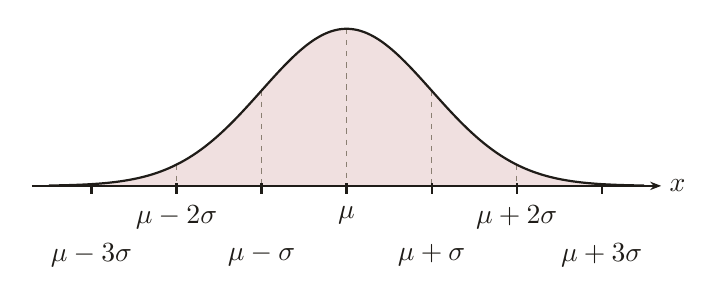
\begin{tikzpicture}[
  x=1.08cm,
  y=5cm,
  every node/.style={font=\normalsize, journalink},
  axis/.style={journalink, line width=0.8pt, -{Stealth[length=4pt]}},
  tick/.style={journalink, line width=0.8pt},
  curve/.style={journalink, line width=0.8pt},
  guide/.style={journalmuted, line width=0.5pt, dash pattern=on 2pt off 2pt},
  region/.style={journalaccent, fill opacity=0.15}
]
  % ---- left edge, right edge and floor, shared with Fig. 4.5 ------------
  \path ([yshift=-1.10cm]-3.75,0) -- ([yshift=-1.10cm]4.10,0);

  % ---- the whole area under the curve ----------------------------------
  \fill[region]
    (-3.5,0) -- (3.5,0) -- (3.5,0.0008727)
    -- plot[domain=3.5:-3.5, samples=300, smooth] (\x,{\normaldensity{\x}})
    -- cycle;

  % ---- the seven boundaries, each from its point on the curve down to the
  %      axis (spec 1.6: they do not run out above the curve) -------------
  \draw[guide] (-3,0.0044318) -- (-3,0);
  \draw[guide] (-2,0.0539910) -- (-2,0);
  \draw[guide] (-1,0.2419707) -- (-1,0);
  \draw[guide] ( 0,0.3989423) -- ( 0,0);
  \draw[guide] ( 1,0.2419707) -- ( 1,0);
  \draw[guide] ( 2,0.0539910) -- ( 2,0);
  \draw[guide] ( 3,0.0044318) -- ( 3,0);

  % ---- density curve ---------------------------------------------------
  \draw[curve] plot[domain=-3.5:3.5, samples=300, smooth]
    (\x,{\normaldensity{\x}});

  % ---- x axis, ticks and staggered labels ------------------------------
  \draw[axis] (-3.7,0) -- (3.7,0);
  \node[anchor=west, inner sep=2.8pt] at (3.7,0) {$x$};

  \foreach \p in {-3,-2,-1,0,1,2,3}
    \draw[tick] ([yshift=0.035cm]\p,0) -- ([yshift=-0.106cm]\p,0);

  % upper row: the even multiples
  \node[anchor=north, inner sep=0pt] at ([yshift=-0.25cm]-2,0)
    {$\mu-2\sigma$};
  \node[anchor=north, inner sep=0pt] at ([yshift=-0.25cm]0,0) {$\mu$};
  \node[anchor=north, inner sep=0pt] at ([yshift=-0.25cm]2,0)
    {$\mu+2\sigma$};
  % lower row: the odd ones
  \node[anchor=north, inner sep=0pt] at ([yshift=-0.73cm]-3,0)
    {$\mu-3\sigma$};
  \node[anchor=north, inner sep=0pt] at ([yshift=-0.73cm]-1,0)
    {$\mu-\sigma$};
  \node[anchor=north, inner sep=0pt] at ([yshift=-0.73cm]1,0)
    {$\mu+\sigma$};
  \node[anchor=north, inner sep=0pt] at ([yshift=-0.73cm]3,0)
    {$\mu+3\sigma$};

\end{tikzpicture}
\end{document}
